\documentclass[aspectratio=169,11pt]{beamer}

\usetheme{Madrid}
\usecolortheme{default}
\setbeamertemplate{navigation symbols}{}
\setbeamertemplate{footline}[frame number]

\usepackage{amsmath,amssymb}
\usepackage{graphicx}
\usepackage{tikz}
\usetikzlibrary{positioning,calc}
\usetikzlibrary{arrows.meta,decorations.pathmorphing}

\definecolor{RamRed}{RGB}{190,40,45}
\definecolor{RamBlue}{RGB}{30,90,180}
\definecolor{SoftGray}{RGB}{245,245,245}
\definecolor{DarkGray}{RGB}{70,70,70}
\definecolor{MapGreen}{RGB}{48,150,95}
\definecolor{MapGold}{RGB}{235,180,45}

\setbeamercolor{title}{fg=DarkGray}
\setbeamercolor{frametitle}{fg=white,bg=RamBlue}
\setbeamercolor{structure}{fg=RamBlue}

\tikzset{
  v/.style={circle,draw=black,fill=white,inner sep=1.8pt},
  edge/.style={draw=RamBlue,line width=1.25pt},
  topic/.style={draw=black!30,fill=SoftGray,rounded corners=5pt,inner sep=7pt,
    text width=5.8cm,minimum height=1.65cm,align=left},
}


\usepackage{booktabs}
\tikzset{dot/.style={circle,fill=black,inner sep=2pt}, lab/.style={circle,draw=black,fill=white,inner sep=2pt,minimum size=6mm,font=\small},selected/.style={draw=RamRed,line width=2pt}}

\newcommand{\Def}[2]{\begin{block}{#1}#2\end{block}}
\newcommand{\Thm}[2]{\begin{block}{#1}#2\end{block}}
\renewcommand{\Proof}[1]{\begin{block}{Proof}\normalsize #1\end{block}}
\newcommand{\Question}[1]{\begin{block}{Question}#1\end{block}}
\renewcommand{\Example}[1]{\begin{block}{Example}#1\end{block}}
\newcommand{\fall}[2]{#1^{\underline{#2}}}
\newcommand{\rise}[2]{#1^{\overline{#2}}}
\newcommand{\stir}[2]{\left\{\begin{matrix}#1\\#2\end{matrix}\right\}}
\newcommand{\cyc}[2]{\left[\begin{matrix}#1\\#2\end{matrix}\right]}
\newcommand{\eul}[2]{\left\langle\begin{matrix}#1\\#2\end{matrix}\right\rangle}
\newcommand{\coef}[2]{[#1^{#2}]}
\newcommand{\gap}{\par\medskip}

\title{Partitions and Special Numbers}
\author{Jeremy Quastel}\date{}\begin{document}
\begin{frame}[plain]\begin{center}{\Huge\bfseries Partitions and Special Numbers}\par\vspace{.25cm}{\Large Section 2.8.1--2.8.5}\par\vspace{.15cm}{\large Harris--Hirst--Mossinghoff, \emph{Combinatorics and Graph Theory}}\par\vspace{.1cm}\resizebox{!}{2.7cm}{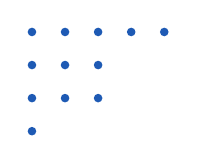
\begin{tikzpicture}[scale=.42]\foreach \y/\n in {0/5,-1/3,-2/3,-3/1}{\foreach \x in {1,...,\n}{\fill[RamBlue](\x,\y)circle(.13);}}\end{tikzpicture}\qquad$12=5+3+3+1$}\par\vspace{.25cm}Jeremy Quastel\end{center}\end{frame}
\begin{frame}[plain]\large \begin{center}{\Huge\bfseries Today\textquotesingle s lecture}\par\vspace{.5cm}\end{center}\begin{columns}[c,onlytextwidth]\begin{column}{.48\textwidth}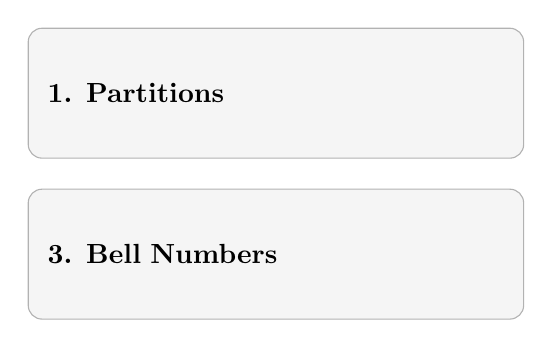
\begin{tikzpicture}\node[topic](a){\textbf{1. Partitions}};\node[topic,below=.38cm of a]{\textbf{3. Bell Numbers}};\end{tikzpicture}\end{column}\begin{column}{.48\textwidth}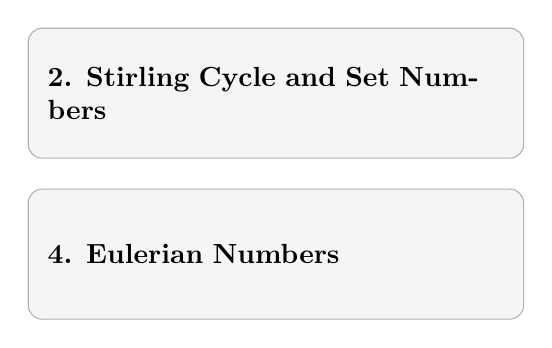
\begin{tikzpicture}\node[topic](a){\textbf{2. Stirling Cycle and Set Numbers}};\node[topic,below=.38cm of a]{\textbf{4. Eulerian Numbers}};\end{tikzpicture}\end{column}\end{columns}\end{frame}
\begin{frame}{Section 2.8.1: Integer partitions}
\large
\Def{Partition of an integer}{A partition of a nonnegative integer $n$ is a multiset of positive integers with sum $n$. Its members are called parts. Let $p(n)$ be the number of partitions of $n$.}
\gap Order does not matter. We normally write the parts in decreasing order. The empty partition gives $p(0)=1$.
\end{frame}
\begin{frame}{The partitions of $5$}
\large
\begin{align*}
5&=5\\&=4+1\\&=3+2\\&=3+1+1\\&=2+2+1\\&=2+1+1+1\\&=1+1+1+1+1.
\end{align*}
\begin{center}$p(5)=7$.\end{center}
\end{frame}
\begin{frame}{Partitions and compositions}
\large
\Def{Composition}{A composition of $n$ is an ordered list of positive integers with sum $n$.}
\gap Thus $3+2$ and $2+3$ are different compositions but the same partition.
\gap For $n\geq1$, there are $2^{n-1}$ compositions: choose where to cut a row of $n$ ones, using any subset of the $n-1$ gaps.
\end{frame}
\begin{frame}{Ferrers diagrams}
\large
\begin{center}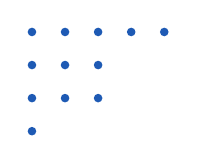
\begin{tikzpicture}[scale=.42]\foreach \y/\n in {0/5,-1/3,-2/3,-3/1}{\foreach \x in {1,...,\n}{\fill[RamBlue](\x,\y)circle(.13);}}\end{tikzpicture}\qquad$12=5+3+3+1$\end{center}
\gap Draw one row of dots for each part, left aligned and ordered from longest to shortest. This represents $12=5+3+3+1$.
\end{frame}
\begin{frame}{Conjugate partitions}
\large
\Def{Conjugation}{Interchange rows and columns of a Ferrers diagram. The column lengths form the conjugate partition.}
\Example{The conjugate of $(5,3,3,1)$ is $(4,3,3,1,1)$.}
\gap Conjugating twice returns to the original partition, so conjugation is a bijection.
\end{frame}
\begin{frame}{A consequence of conjugation}
\large
\Thm{Theorem}{The number of partitions of $n$ into exactly $k$ parts equals the number of partitions of $n$ whose largest part is $k$.}
\Proof{A Ferrers diagram with $k$ rows becomes a diagram whose longest row has $k$ dots.}
\gap Similarly, at most $k$ parts corresponds to largest part at most $k$.
\end{frame}
\begin{frame}{Partitions with exactly $k$ parts}
\large
\Def{Notation}{Let $p_k(n)$ be the number of partitions of $n$ into exactly $k$ positive parts. Set $p_0(0)=1$, and use zero for impossible parameters.}
\Thm{Recurrence}{For $n,k\geq1$,
\[p_k(n)=p_{k-1}(n-1)+p_k(n-k).\]}
\end{frame}
\begin{frame}{Proof of the partition recurrence}
\large
\Proof{Separate partitions into two cases.\gap If a part equals $1$, remove one such part. This is a bijection with partitions of $n-1$ into $k-1$ parts.\gap If every part is at least $2$, subtract $1$ from each of the $k$ parts. This is a bijection with partitions of $n-k$ into $k$ positive parts.}
\end{frame}
\begin{frame}{The partition generating function}
\large
\Thm{Identity}{\[\sum_{n\geq0}p(n)x^n=\prod_{j\geq1}\frac1{1-x^j}.\]}
\Proof{The factor $1+x^j+x^{2j}+\cdots$ chooses the number of parts equal to $j$. Multiplying chooses all multiplicities, and the exponent records their sum.}
\end{frame}
\begin{frame}{Why the infinite product is well defined}
\large
\gap To find the coefficient of $x^n$, only factors with $j\leq n$ can contribute a positive power.
\gap Therefore each coefficient requires only finitely many factors and finitely many choices.
\gap For largest part at most $k$, the generating function is the finite product $\prod_{j=1}^k(1-x^j)^{-1}$.
\end{frame}
\begin{frame}{Exactly $k$ parts: generating function}
\large
\Thm{Identity}{\[\sum_{n\geq0}p_k(n)x^n=\frac{x^k}{(1-x)(1-x^2)\cdots(1-x^k)}.\]}
\Proof{Subtract $1$ from each of $k$ parts, allowing zeros. After discarding zeros, this gives a partition into at most $k$ parts. Conjugation converts this to a partition with largest part at most $k$.}
\end{frame}
\begin{frame}{Distinct parts and odd parts}
\large
\Thm{Euler's partition theorem}{The number of partitions of $n$ into distinct parts equals the number of partitions of $n$ into odd parts.}
\gap For $n=5$, distinct-part partitions are $5$, $4+1$, $3+2$. Odd-part partitions are $5$, $3+1+1$, $1+1+1+1+1$.
\end{frame}
\begin{frame}{A generating-function proof}
\large
\Proof{Distinct parts contribute
\[\prod_{j\geq1}(1+x^j)=\prod_{j\geq1}\frac{1-x^{2j}}{1-x^j}.
\]
Cancel the even-indexed denominator factors to obtain
\[\prod_{\substack{j\geq1\\j\text{ odd}}}\frac1{1-x^j},\]
which counts partitions into odd parts. Cancellation is valid coefficient by coefficient.}
\end{frame}
\begin{frame}{A direct bijection}
\large
\Proof{In a partition into odd parts, write the multiplicity of each odd part $u$ in binary. Replace $2^j$ copies of $u$ by the single part $2^ju$ whenever the corresponding binary digit is $1$.\gap The resulting parts are distinct, because each positive integer has a unique odd part and power of $2$. Splitting each distinct part back into copies of its odd part reverses the construction.}
\end{frame}
\begin{frame}{A partition example}
\large
\Example{Start with the odd-part partition
\[3+3+3+1+1+1+1+1.\]
Three copies of $3$ become $6+3$, and five copies of $1$ become $4+1$. The distinct-part partition is
\[6+4+3+1.\]}
\end{frame}
\begin{frame}{Section 2.8.2: Stirling cycle numbers}
\large
\Def{Definition}{The unsigned Stirling cycle number
\[\cyc nk\]
counts permutations of $[n]$ with exactly $k$ cycles, including fixed points.}
\gap Cycles are unordered, and writing a cycle from a different starting point does not change it.
\end{frame}
\begin{frame}{An example with three elements}
\large
\begin{center}\renewcommand{\arraystretch}{1.5}
\begin{tabular}{ccl}
Cycles & Count & Permutations\\\hline
1&2&$(123),(132)$\\
2&3&$(12)(3),(13)(2),(23)(1)$\\
3&1&$(1)(2)(3)$
\end{tabular}\end{center}
\[\cyc31=2,\qquad\cyc32=3,\qquad\cyc33=1.\]
\end{frame}
\begin{frame}{Boundary values}
\large
\[\cyc00=1,\qquad\cyc n0=0\ (n>0),\qquad\cyc nn=1.\]
\gap For $n\geq1$,
\[\cyc n1=(n-1)!.\]
\gap A single cycle is a circular arrangement of all $n$ elements.
\end{frame}
\begin{frame}{The cycle-number recurrence}
\large
\Thm{Recurrence}{For $n\geq1$,
\[\cyc nk=\cyc{n-1}{k-1}+(n-1)\cyc{n-1}k.\]}
\gap Distinguish whether $n$ is a one-cycle or belongs to a longer cycle.
\end{frame}
\begin{frame}{Proof of the cycle recurrence}
\large
\Proof{If $(n)$ is a cycle by itself, the other elements form a permutation with $k-1$ cycles.\gap Otherwise remove $n$ from its cycle, leaving a permutation of $n-1$ elements with $k$ cycles. Conversely, insert $n$ immediately after any of the $n-1$ elements in its cycle notation.\gap These disjoint cases give the recurrence.}
\end{frame}
\begin{frame}{A small cycle-number table}
\large
\begin{center}\renewcommand{\arraystretch}{1.5}
\begin{tabular}{c|rrrrr}
$n\backslash k$&1&2&3&4&5\\\hline
1&1\\2&1&1\\3&2&3&1\\4&6&11&6&1\\5&24&50&35&10&1
\end{tabular}\end{center}
\gap The row for $n$ sums to $n!$.
\end{frame}
\begin{frame}{Rising factorials}
\large
\Def{Notation}{\[\rise xn=x(x+1)\cdots(x+n-1),\qquad\rise x0=1.\]}
\Thm{Identity}{\[\rise xn=\sum_{k=0}^n\cyc nkx^k.\]}
\end{frame}
\begin{frame}{Proof of the rising-factorial identity}
\large
\Proof{Write $P_n(x)=\sum_k\cyc nkx^k$. Multiply the recurrence by $x^k$ and sum:
\[P_n(x)=xP_{n-1}(x)+(n-1)P_{n-1}(x).
\]
Since $P_0(x)=1$, induction gives
\[P_n(x)=x(x+1)\cdots(x+n-1).\]}
\end{frame}
\begin{frame}{Section 2.8.3: Stirling set numbers}
\large
\Def{Definition}{The Stirling set number
\[\stir nk\]
counts partitions of the set $[n]$ into $k$ nonempty, unlabeled blocks.}
\gap Here the elements being partitioned are distinct. This differs from partitioning the integer $n$ into part sizes.
\end{frame}
\begin{frame}{A set-partition example}
\large
The partitions of $\{1,2,3\}$ into two blocks are
\[\{\{1\},\{2,3\}\},\quad\{\{2\},\{1,3\}\},\quad\{\{3\},\{1,2\}\}.\]
\gap Thus $\stir32=3$.
\gap The order of the blocks and the order of elements within each block do not matter.
\end{frame}
\begin{frame}{The set-number recurrence}
\large
\Thm{Recurrence}{\[\stir nk=\stir{n-1}{k-1}+k\stir{n-1}k.\]}
\Proof{If $\{n\}$ is a singleton block, partition the other elements into $k-1$ blocks. Otherwise partition the other elements into $k$ blocks and choose one of these $k$ blocks to receive $n$.}
\end{frame}
\begin{frame}{A small set-number table}
\large
\begin{center}\renewcommand{\arraystretch}{1.5}
\begin{tabular}{c|rrrrr}
$n\backslash k$&1&2&3&4&5\\\hline
1&1\\2&1&1\\3&1&3&1\\4&1&7&6&1\\5&1&15&25&10&1
\end{tabular}\end{center}
\gap Boundary values: $\stir00=1$, $\stir n0=0$ for $n>0$, and $\stir nn=1$.
\end{frame}
\begin{frame}{Surjections and set partitions}
\large
\Thm{Identity}{The number of onto functions from $[n]$ to $[k]$ is
\[k!\stir nk.\]}
\Proof{The nonempty inverse images of target elements form $k$ blocks. Conversely, partition $[n]$ into $k$ blocks, then assign the $k$ distinct target labels to the blocks.}
\end{frame}
\begin{frame}{An explicit formula}
\large
\Thm{Formula}{For $n,k\geq1$,
\[\stir nk=\frac1{k!}\sum_{j=0}^k(-1)^j\binom kj(k-j)^n.\]}
\Proof{Use the inclusion--exclusion formula for surjections and divide by the $k!$ ways to label the blocks.}
\end{frame}
\begin{frame}{Two-block partitions}
\large
\Thm{Identity}{For $n\geq1$,
\[\stir n2=2^{n-1}-1.\]}
\Proof{Choose a nonempty proper subset as one block: $2^n-2$ choices. Each partition is counted twice, once for either block. Divide by $2$.}
\end{frame}
\begin{frame}{Powers and falling factorials}
\large
\Thm{Identity}{\[x^n=\sum_{k=0}^n\stir nk\fall xk.\]}
\Proof{For a nonnegative integer $x$, count functions from $[n]$ to $[x]$ by image size $k$. Partition the domain into its $k$ nonempty fibers, then assign distinct target values to the blocks in $\fall xk$ ways.\gap Since both sides are polynomials agreeing at all nonnegative integers, the identity holds for every $x$.}
\end{frame}
\begin{frame}{Comparing the two Stirling families}
\large
\begin{center}\renewcommand{\arraystretch}{1.7}
\begin{tabular}{lcc}
& Cycle numbers & Set numbers\\\hline
Object & Permutations & Set partitions\\
Parameter $k$ & Number of cycles & Number of blocks\\
Insertion choices & $n-1$ & $k$\\
Row sum & $n!$ & $B_n$
\end{tabular}\end{center}
\gap Both recurrences separate off the case where the new element stands alone.
\end{frame}
\begin{frame}{Section 2.8.4: Bell numbers}
\large
\Def{Bell number}{The Bell number $B_n$ counts all partitions of an $n$-element set. Thus
\[B_n=\sum_{k=0}^n\stir nk.\]}
\[B_0,B_1,B_2,B_3,B_4,B_5=1,1,2,5,15,52.\]
\end{frame}
\begin{frame}{A Bell-number recurrence}
\large
\Thm{Recurrence}{\[B_{n+1}=\sum_{k=0}^n\binom nkB_k.\]}
\Proof{In a partition of $[n+1]$, consider the block containing $n+1$. Choose the $k$ elements outside that block, then partition those elements in $B_k$ ways. The remaining elements all belong to the distinguished block.}
\end{frame}
\begin{frame}{Computing a Bell number}
\large
\begin{align*}
B_4&=\binom30B_0+\binom31B_1+\binom32B_2+\binom33B_3\\
&=1+3+6+5=15.
\end{align*}
\gap This recurrence computes Bell numbers without first constructing the entire Stirling table.
\end{frame}
\begin{frame}{Exponential generating functions}
\large
\Def{Definition}{The exponential generating function of $(a_n)$ is
\[\widehat A(x)=\sum_{n\geq0}a_n\frac{x^n}{n!}.\]}
\gap The factorial denominators are useful for objects built on labeled sets. Binomial convolution becomes multiplication of exponential generating functions.
\end{frame}
\begin{frame}{The Bell exponential generating function}
\large
\Thm{Identity}{\[\sum_{n\geq0}B_n\frac{x^n}{n!}=\exp(e^x-1).\]}
\Proof{The Bell recurrence implies $\widehat B'(x)=e^x\widehat B(x)$, with $\widehat B(0)=1$. Solving this differential equation gives $\widehat B(x)=\exp(e^x-1)$.}
\end{frame}
\begin{frame}{Dobinski's formula}
\large
\Thm{Formula}{For $n\geq1$,
\[B_n=\frac1e\sum_{m=0}^{\infty}\frac{m^n}{m!}.\]}
\Proof{Use $m^n=\sum_k\stir nk\fall mk$. For each $k$,
\[\sum_{m\geq0}\frac{\fall mk}{m!}=\sum_{m\geq k}\frac1{(m-k)!}=e.\]
The finite sum over $k$ then gives $eB_n$.}
\end{frame}
\begin{frame}{Section 2.8.5: Eulerian numbers}
\large
\Def{Ascent}{An ascent of a permutation $a_1\cdots a_n$ is an index $i$ such that $a_i<a_{i+1}$.}
\Def{Eulerian number}{Write $\eul nk$ for the number of permutations of $[n]$ with exactly $k$ ascents.}
\gap Counting descents instead gives the same numbers, by reversing the order of a permutation.
\end{frame}
\begin{frame}{An Eulerian example}
\large
\begin{center}\renewcommand{\arraystretch}{1.5}
\begin{tabular}{ccl}
Ascents & Count & Permutations\\\hline
0&1&321\\
1&4&132, 213, 231, 312\\
2&1&123
\end{tabular}\end{center}
\[\eul30=1,\qquad\eul31=4,\qquad\eul32=1.\]
\end{frame}
\begin{frame}{The Eulerian recurrence}
\large
\Thm{Recurrence}{For $n\geq2$,
\[\eul nk=(k+1)\eul{n-1}k+(n-k)\eul{n-1}{k-1}.\]}
\gap Use $\eul10=1$, and interpret entries outside $0\leq k\leq n-1$ as zero.
\end{frame}
\begin{frame}{Insertion positions that preserve ascents}
\large
\Proof{Start with a permutation of $[n-1]$ having $k$ ascents and insert the largest element $n$.\gap Inserting at the beginning adds no ascent. Inserting in any existing ascent replaces that ascent by one ascent and one descent, preserving the count.\gap These $k+1$ positions give the first term of the recurrence.}
\end{frame}
\begin{frame}{Insertion positions that add an ascent}
\large
\Proof{Start instead with a permutation having $k-1$ ascents. There are $n$ insertion positions in total. Exactly $k$ preserve the ascent count, by the preceding argument.\gap The remaining $n-k$ positions increase the number of ascents by one: insert at the end or into a descent.\gap These give the second term. Every permutation of $[n]$ is recovered uniquely by deleting $n$.}
\end{frame}
\begin{frame}{An Eulerian triangle}
\large
\begin{center}\renewcommand{\arraystretch}{1.5}
\begin{tabular}{c|rrrrr}
$n\backslash k$&0&1&2&3&4\\\hline
1&1\\2&1&1\\3&1&4&1\\4&1&11&11&1\\5&1&26&66&26&1
\end{tabular}\end{center}
\gap Each row sums to $n!$, since every permutation has some number of ascents.
\end{frame}
\begin{frame}{Eulerian symmetry}
\large
\Thm{Identity}{\[\eul nk=\eul n{n-1-k}.\]}
\Proof{Replace each value $a_i$ by $n+1-a_i$. Every ascent becomes a descent and every descent becomes an ascent. This operation is its own inverse.}
\gap The extreme entries are both $1$, corresponding to decreasing and increasing permutations.
\end{frame}
\begin{frame}{Eulerian polynomials}
\large
\Def{Definition}{For $n\geq1$, set
\[A_n(x)=\sum_{k=0}^{n-1}\eul nkx^k.\]}
\Thm{Recurrence}{\[A_n(x)=(1+(n-1)x)A_{n-1}(x)+x(1-x)A'_{n-1}(x).\]}
\gap Multiply the Eulerian-number recurrence by $x^k$ and sum over $k$.
\end{frame}
\begin{frame}{Power sums as a generating function}
\large
\Thm{Identity}{For $n\geq1$,
\[\sum_{m\geq0}m^nx^m=\frac{xA_n(x)}{(1-x)^{n+1}}.\]}
\Proof{For $n=1$, differentiate the geometric series. Applying $x\,d/dx$ multiplies the coefficient of $x^m$ by $m$. Differentiating the right-hand side produces exactly the Eulerian-polynomial recurrence.}
\end{frame}
\begin{frame}{An explicit Eulerian formula}
\large
\Thm{Formula}{For $0\leq k\leq n-1$,
\[\eul nk=\sum_{j=0}^{k+1}(-1)^j\binom{n+1}j(k+1-j)^n.\]}
\Proof{Multiply the preceding generating-function identity by $(1-x)^{n+1}$ and compare coefficients of $x^{k+1}$.}
\end{frame}
\begin{frame}{An Eulerian calculation}
\large
For $n=4,k=1$,
\[\eul41=2^4-\binom511^4+\binom520^4=16-5=11.\]
\gap The recurrence gives the same result:
\[\eul41=2\eul31+3\eul30=8+3=11.\]
\end{frame}
\begin{frame}{Practice: identify the family}
\large
\Question{Which number counts each of the following?}
\begin{enumerate}
\item Ways to write $8$ as an unordered sum of positive integers.
\item Permutations of $[8]$ with three cycles.
\item Partitions of $[8]$ into three nonempty blocks.
\item All partitions of $[8]$.
\item Permutations of $[8]$ with three ascents.
\end{enumerate}
\end{frame}
\begin{frame}{Practice: answers}
\large
\begin{center}\renewcommand{\arraystretch}{1.6}
\begin{tabular}{lc}
Integer partitions & $p(8)$\\
Permutations with three cycles & $\cyc83$\\
Set partitions into three blocks & $\stir83$\\
All set partitions & $B_8$\\
Permutations with three ascents & $\eul83$
\end{tabular}\end{center}
\end{frame}
\begin{frame}{Summary}
\large
\begin{itemize}
\item Integer partitions are counted by products recording part multiplicities.
\item Stirling cycle and set numbers distinguish cycles from blocks.
\item Bell numbers sum over all possible numbers of blocks.
\item Eulerian numbers count ascent patterns and appear in power-sum generating functions.
\end{itemize}
\end{frame}
\begin{frame}{Next time: Course Review}\begin{center}{\Huge Course Review}\end{center}\end{frame}
\end{document}